\documentclass[aspectratio=169,14pt]{beamer}
\usetheme{default}
\usepackage{fontspec}
\setmainfont{texgyrepagella-regular.otf}[BoldFont=texgyrepagella-bold.otf,ItalicFont=texgyrepagella-italic.otf,BoldItalicFont=texgyrepagella-bolditalic.otf]
\setsansfont{texgyreheros-regular.otf}[BoldFont=texgyreheros-bold.otf,ItalicFont=texgyreheros-italic.otf,BoldItalicFont=texgyreheros-bold.otf,BoldItalicFeatures={FakeSlant=0.2}]
\setmonofont{lmmono10-regular.otf}[Scale=0.85]
\setbeamertemplate{navigation symbols}{}
\usepackage{pgfpages}
\newif\ifpresenter
\ifdefined\PresenterVersion\presentertrue\else\presenterfalse\fi
\ifpresenter
  \setbeameroption{show notes on second screen=right}
  \setbeamertemplate{note page}[plain]
\fi
\usepackage{amsmath,amssymb,bm,booktabs,array,graphicx,xcolor}
\usepackage{tikz,pgfplots,adjustbox,listings,xurl}
\pgfplotsset{compat=1.18}
\usetikzlibrary{arrows.meta,positioning,calc,fit,shapes.geometric,decorations.pathreplacing,patterns}
% UIUC official brand colors, verified 2026-10-23.
% https://brand.illinois.edu/visual-identity/color
\definecolor{IlliniOrange}{HTML}{FF5F05}
\definecolor{IlliniBlue}{HTML}{13294B}
\definecolor{Storm}{HTML}{707372}
\definecolor{LightStorm}{HTML}{C6C7C6}
\definecolor{Industrial}{HTML}{1D58A7}
\definecolor{Patina}{HTML}{007E8E}
\tikzset{>=Stealth, every node/.style={font=\small,text=IlliniBlue}, box/.style={draw=IlliniBlue,rounded corners=2pt,align=center,inner sep=6pt,execute at begin node=\hyphenpenalty10000\relax}, orangebox/.style={box,draw=IlliniOrange,very thick}, edge/.style={->,thick,IlliniBlue}, accent/.style={->,very thick,IlliniOrange}}
\pgfplotsset{every axis/.append style={width=13.5cm,height=6.5cm,axis line style={IlliniBlue},tick label style={font=\small,text=IlliniBlue},label style={font=\small,text=IlliniBlue},legend style={font=\small,draw=none,fill=white},grid style={LightStorm},major grid style={LightStorm},axis lines=left,clip=false}, every axis plot/.append style={thick}}

\definecolor{slidepaper}{RGB}{234,220,201}
\setbeamercolor{background canvas}{bg=slidepaper}
\setbeamercolor{normal text}{fg=IlliniBlue}
\setbeamercolor{frametitle}{fg=IlliniBlue}
\setbeamercolor{title}{fg=IlliniBlue}
\setbeamercolor{item}{fg=IlliniOrange}
\setbeamerfont{frametitle}{size=\large,series=\bfseries}
\setbeamerfont{title}{size=\Large,series=\bfseries}
\setbeamertemplate{itemize item}{\color{IlliniOrange}$\bullet$}
\setbeamertemplate{itemize subitem}{\color{IlliniOrange}\footnotesize$\circ$}
\setbeamercolor{orangerule}{bg=IlliniOrange}
\setbeamertemplate{headline}{\begin{beamercolorbox}[wd=\paperwidth,ht=0.1cm,dp=0.1cm]{orangerule}\end{beamercolorbox}}
\setbeamertemplate{footline}{\begin{beamercolorbox}[wd=\paperwidth,ht=0.1cm,dp=0.1cm]{orangerule}\end{beamercolorbox}}
\setbeamersize{text margin left=0.65cm,text margin right=0.65cm}
\setlength{\leftmargini}{1.1em}
\newenvironment{slidebullets}{\begin{itemize}\setlength\itemsep{0.8em}}{\end{itemize}}
\pgfplotsset{every axis/.append style={legend style={fill=slidepaper}}}
\lstdefinelanguage{CoursePython}{keywords={from,import,for,in,if,else,def,return,assert,True,False,None},sensitive=true,morecomment=[l]{\#},morestring=[b]',morestring=[b]"}
\lstset{language=CoursePython,basicstyle=\ttfamily\small,keywordstyle=\color{IlliniBlue}\bfseries,commentstyle=\color{Storm},stringstyle=\color{IlliniBlue},showstringspaces=false,breaklines=true,columns=fullflexible,keepspaces=true,frame=none,aboveskip=0.7em,belowskip=0.7em}
\newcommand{\E}{\mathbb E}
\newcommand{\Var}{\operatorname{Var}}
\newcommand{\Cov}{\operatorname{Cov}}
\hypersetup{colorlinks=true,urlcolor=IlliniBlue,linkcolor=IlliniBlue}

\title{Marketing Analytics}
\subtitle{Visualization and Data Quality}
\author{By Nathan Yang}
\date{Session 03}
\begin{document}
\begin{frame}
\titlepage
\end{frame}
\begin{frame}{A Campaign Comparison}
\usebeamercolor[fg]{normal text}
\vfill
\begin{slidebullets}
\item Campaign B converts more new and returning customers within each group.
\item Its aggregate conversion rate is lower.
\item The customer mix determines which comparison the aggregate makes.
\end{slidebullets}
\vfill
\note{The synthetic campaigns differ in the proportion of returning customers. The group rates and the aggregate can move in opposite directions without an arithmetic error.

M2, Section 2.3, Marketing Analytics Lecture Notes. \url{../06_Lecture_Notes/modules/M02_Customer_Data_and_Visualization.md}}
\end{frame}
\begin{frame}{Customer Mix Reverses the Ranking}
\usebeamercolor[fg]{normal text}
\centering
\begingroup
\begin{adjustbox}{max width=0.98\textwidth,max totalheight=0.65\textheight}
% Original synthetic teaching figure; see corresponding module.
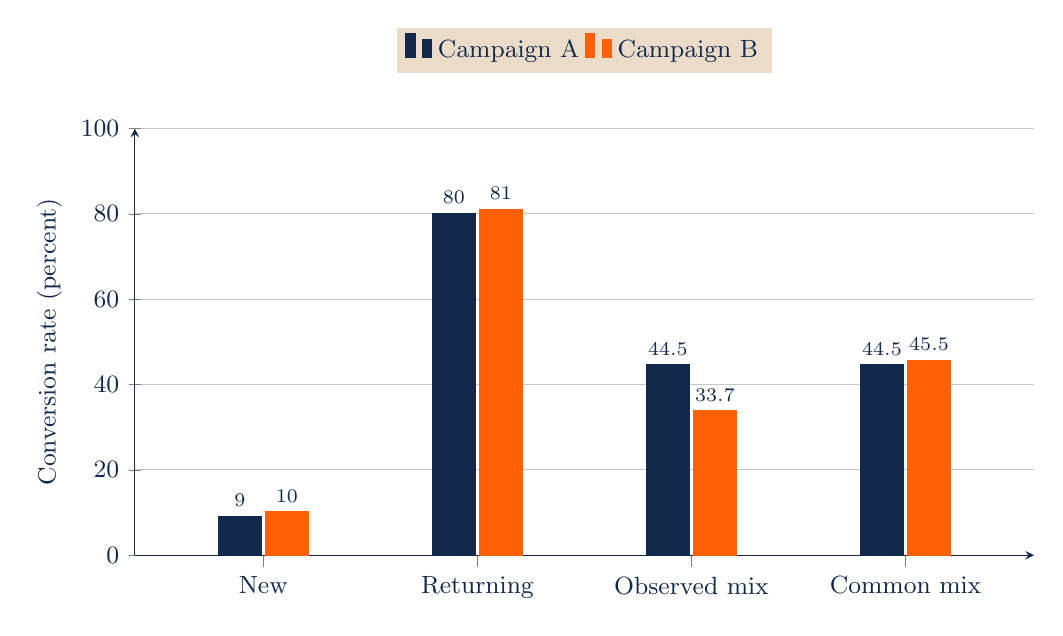
\begin{tikzpicture}
\begin{axis}[ybar,bar width=15pt,width=13cm,height=7cm,ymin=0,ymax=100,xmin=.4,xmax=4.6,xtick={1,2,3,4},xticklabels={New,Returning,Observed mix,Common mix},ylabel={Conversion rate (percent)},ytick={0,20,40,60,80,100},ymajorgrids=true,legend style={at={(.5,1.13)},anchor=south,legend columns=2},nodes near coords,nodes near coords style={font=\scriptsize},every node near coord/.append style={/pgf/number format/fixed,/pgf/number format/precision=1}]
\addplot[fill=IlliniBlue,draw=IlliniBlue] coordinates {(1,9)(2,80)(3,44.5)(4,44.5)};
\addplot[fill=IlliniOrange,draw=IlliniOrange] coordinates {(1,10)(2,81)(3,33.6667)(4,45.5)};
\legend{Campaign A,Campaign B}
\end{axis}
\end{tikzpicture}

\end{adjustbox}
\endgroup
\par\medskip
{\small Synthetic campaigns. Both within-group rates rise by one percentage point.\par}
\note{Standardization holds group weights fixed. It supplies a common-population descriptive comparison. Causal interpretation would require evidence about assignment and comparability within groups.

M2, Section 2.3, Marketing Analytics Lecture Notes. \url{../06_Lecture_Notes/modules/M02_Customer_Data_and_Visualization.md}}
\end{frame}
\begin{frame}{A Standardized Conversion Rate}
\usebeamercolor[fg]{normal text}
\noindent Use common customer-group weights $w_g$ for each campaign $c$.
\medskip
\[
\bar p_c^{\mathrm{std}}=\sum_g w_g p_{cg},\qquad \sum_g w_g=1
\]
\medskip
\noindent Changing the weights changes the population represented by the rate.
\note{The same weights should apply to every campaign in the stated comparison. The group-specific rates can still reflect selection or other differences within groups.

M2, Section 2.3, Marketing Analytics Lecture Notes. \url{../06_Lecture_Notes/modules/M02_Customer_Data_and_Visualization.md}}
\end{frame}
\begin{frame}{Chart Choice Follows the Question}
\usebeamercolor[fg]{normal text}
\vfill
\begin{slidebullets}
\item Aligned positions compare magnitudes.
\item Lines compare changes over ordered time.
\item Distributions reveal spread and concentration.
\item Paired displays preserve within-customer changes.
\end{slidebullets}
\vfill
\note{A mean alone can hide whether a change is widespread or concentrated in a small set of customers. Chart choice should follow the estimand and the decision.

M2, Section 2.5, Marketing Analytics Lecture Notes. \url{../06_Lecture_Notes/modules/M02_Customer_Data_and_Visualization.md}}
\end{frame}
\begin{frame}{A Mean Decline Can Hide a Stable Median}
\usebeamercolor[fg]{normal text}
\centering
\begingroup
\begin{adjustbox}{max width=0.98\textwidth,max totalheight=0.65\textheight}
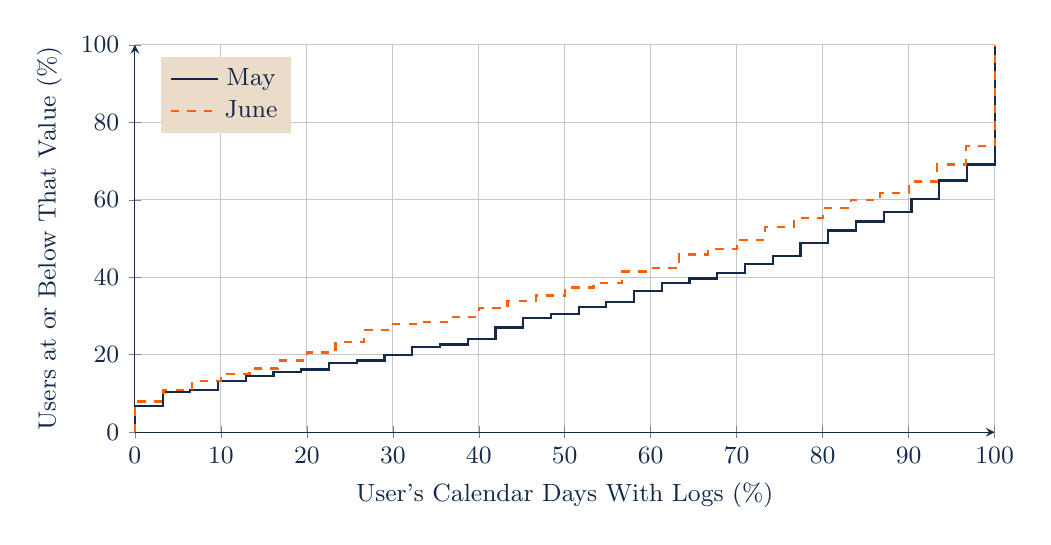
\begin{tikzpicture}
\begin{axis}[width=12.5cm,height=6.5cm,xmin=0,xmax=100,ymin=0,ymax=100,
 xlabel={User's Calendar Days With Logs (\%)},ylabel={Users at or Below That Value (\%)},
 legend style={at={(0.03,0.97)},anchor=north west},grid=major]
\addplot[IlliniBlue,solid,const plot] coordinates {(0,0) (0.00000000,6.76470588) (3.22580645,10.29411765) (6.45161290,10.88235294) (9.67741935,13.23529412) (12.90322581,14.41176471) (16.12903226,15.58823529) (19.35483871,16.17647059) (22.58064516,17.94117647) (25.80645161,18.52941176) (29.03225806,20.00000000) (32.25806452,22.05882353) (35.48387097,22.64705882) (38.70967742,24.11764706) (41.93548387,27.05882353) (45.16129032,29.41176471) (48.38709677,30.58823529) (51.61290323,32.35294118) (54.83870968,33.52941176) (58.06451613,36.47058824) (61.29032258,38.52941176) (64.51612903,39.70588235) (67.74193548,41.17647059) (70.96774194,43.52941176) (74.19354839,45.58823529) (77.41935484,48.82352941) (80.64516129,52.05882353) (83.87096774,54.41176471) (87.09677419,56.76470588) (90.32258065,60.29411765) (93.54838710,65.00000000) (96.77419355,69.11764706) (100.00000000,100.00000000)};
\addplot[IlliniOrange,dashed,const plot] coordinates {(0,0) (0.00000000,7.94117647) (3.33333333,10.88235294) (6.66666667,13.23529412) (10.00000000,15.00000000) (13.33333333,16.47058824) (16.66666667,18.52941176) (20.00000000,20.58823529) (23.33333333,23.23529412) (26.66666667,26.47058824) (30.00000000,27.94117647) (33.33333333,28.52941176) (36.66666667,29.70588235) (40.00000000,32.05882353) (43.33333333,33.82352941) (46.66666667,35.29411765) (50.00000000,37.35294118) (53.33333333,38.52941176) (56.66666667,41.47058824) (60.00000000,42.35294118) (63.33333333,45.88235294) (66.66666667,47.35294118) (70.00000000,49.70588235) (73.33333333,52.94117647) (76.66666667,55.29411765) (80.00000000,57.94117647) (83.33333333,60.00000000) (86.66666667,61.76470588) (90.00000000,64.70588235) (93.33333333,69.11764706) (96.66666667,73.82352941) (100.00000000,100.00000000)};
\legend{May,June}
\end{axis}
\end{tikzpicture}

\end{adjustbox}
\endgroup
\par\medskip
{\small mHealth comparison uses paired customers and a common observation window.\par}
\note{Distribution spread describes variation among customer outcomes. Uncertainty about an average describes how precisely that average is estimated. They require different displays.

M2, Section 2.14.2, Marketing Analytics Lecture Notes. \url{../06_Lecture_Notes/modules/M02_Customer_Data_and_Visualization.md}}
\end{frame}
\begin{frame}{Uncertainty and Dependence}
\usebeamercolor[fg]{normal text}
\vfill
\begin{slidebullets}
\item Repeated days for one customer share common influences.
\item Customer-level resampling preserves each customer history.
\item A confidence interval and a percentile range describe different objects.
\end{slidebullets}
\vfill
\note{An independent-day bootstrap treats days as separate sampling units and can understate uncertainty when observations within a user are correlated. A paired difference should also preserve the pairing.

M3, Section 3.6.1, Marketing Analytics Lecture Notes. \url{../06_Lecture_Notes/modules/M03_Regression.md}}
\end{frame}
\begin{frame}{Nutrition Knowledge and Measurement}
\usebeamercolor[fg]{normal text}
\vfill
\begin{slidebullets}
\item A recorded food log can omit meals and portions.
\item Energy plausibility depends on the measurement instrument and physiology.
\item Age, body size, activity, and recording duration affect screening.
\end{slidebullets}
\vfill
\note{These records contain perturbed weights and undocumented source codes. The course example does not treat an undocumented gender code as validated physiological sex or a goal code as measured activity.

M2, Section 2.11, Marketing Analytics Lecture Notes. \url{../06_Lecture_Notes/modules/M02_Customer_Data_and_Visualization.md}}
\end{frame}
\begin{frame}{Sample Restrictions Change the Comparison}
\usebeamercolor[fg]{normal text}
\centering
\begingroup
\begin{adjustbox}{max width=0.98\textwidth,max totalheight=0.65\textheight}
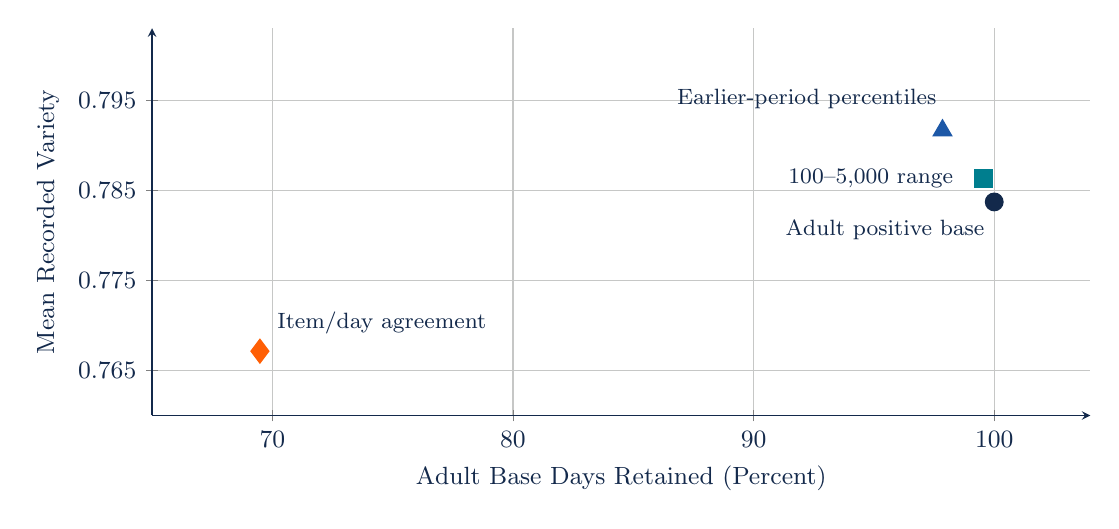
\begin{tikzpicture}
\begin{axis}[xlabel={Adult Base Days Retained (Percent)},ylabel={Mean Recorded Variety},xmin=65,xmax=104,ymin=.76,ymax=.803,xtick={70,80,90,100},ytick={.765,.775,.785,.795},yticklabel style={/pgf/number format/fixed,/pgf/number format/precision=3},grid=major]
\addplot[only marks,mark=*,mark size=3pt,IlliniBlue] coordinates {(100,.7837115)};
\addplot[only marks,mark=square*,mark size=3pt,Patina] coordinates {(99.5623,.7862868)};
\addplot[only marks,mark=triangle*,mark size=3.5pt,Industrial] coordinates {(97.8498,.7916456)};
\addplot[only marks,mark=diamond*,mark size=4pt,IlliniOrange] coordinates {(69.4839,.7671419)};
\node[anchor=north east,font=\footnotesize] at (axis cs:100,.7828) {Adult positive base};
\node[anchor=east,font=\footnotesize] at (axis cs:98.7,.7863) {100--5,000 range};
\node[anchor=south east,font=\footnotesize] at (axis cs:98,.793) {Earlier-period percentiles};
\node[anchor=south west,font=\footnotesize] at (axis cs:69.8,.768) {Item/day agreement};
\end{axis}
\end{tikzpicture}

\end{adjustbox}
\endgroup
\par\medskip
{\small mHealth screening alternatives are explicit analysis choices.\par}
\note{An imposed calorie range is a sensitivity analysis, not an individual diagnosis of adequate intake. Report the observations retained under each rule and compare the resulting estimands.

M2, Section 2.11, Marketing Analytics Lecture Notes. \url{../06_Lecture_Notes/modules/M02_Customer_Data_and_Visualization.md}}
\end{frame}
\begin{frame}{Access Changes the Evidence Sample}
\usebeamercolor[fg]{normal text}
\centering
\begingroup
\fontsize{11}{13.2}\selectfont
\def\small{\fontsize{10}{12}\selectfont}
\def\footnotesize{\fontsize{9}{11}\selectfont}
\def\scriptsize{\fontsize{8}{9.5}\selectfont}
\hyphenpenalty=10000
\begin{adjustbox}{max width=0.98\textwidth,max totalheight=0.65\textheight}
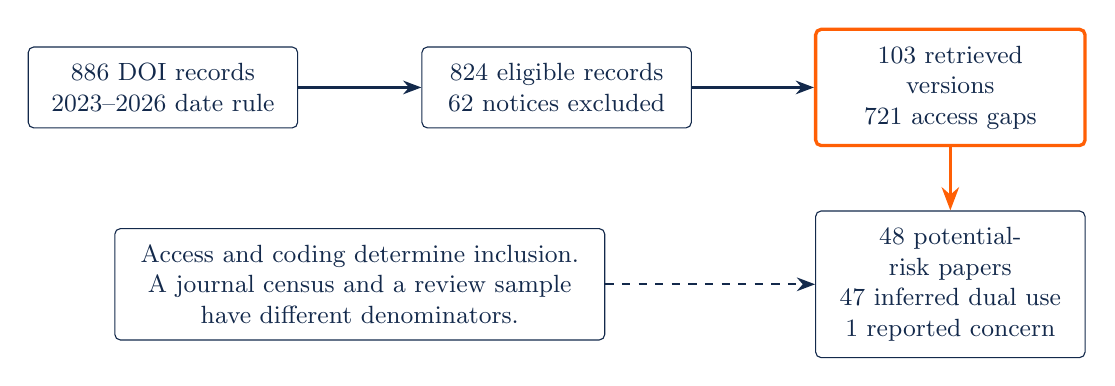
\begin{tikzpicture}
\node[box,text width=3.0cm] (census) at (0,0) {886 DOI records\\2023--2026 date rule};
\node[box,text width=3.0cm] (eligible) at (5.0,0) {824 eligible records\\62 notices excluded};
\node[orangebox,text width=3.0cm] (retrieved) at (10.0,0) {103 retrieved versions\\721 access gaps};
\node[box,text width=3.0cm] (coded) at (10,-2.5) {48 potential-risk papers\\47 inferred dual use\\1 reported concern};
\node[box,text width=5.8cm] (unknown) at (2.5,-2.5) {Access and coding determine inclusion.\\A journal census and a review sample\\have different denominators.};
\draw[edge] (census)--(eligible);
\draw[edge] (eligible)--(retrieved);
\draw[accent] (retrieved)--(coded);
\draw[edge,dashed] (unknown.east)--(coded.west);
\end{tikzpicture}

\end{adjustbox}
\endgroup
\par\medskip
{\small November 5, 2026 snapshot. Counts refer to DOI records and retrieved versions.\par}
\note{The primary mechanism sample includes 47 potential-dual-use reviews and one reported choice concern. Abstract-only papers selected for teaching enter a separate sensitivity sample. Unreviewed papers retain missing codes. The complete coverage calculation appears in M2 Section 2.20.

\url{../01_Resources/13_Consumer_Agency_and_Recent_Research/README.md}}
\end{frame}
\begin{frame}{Selected Findings at a Fixed Date}
\usebeamercolor[fg]{normal text}
\vfill
\centering
{\small\begin{tabular}{lr}
\toprule
Published Category & Claims \\
\midrule
Expired & 22 \\
Weakened & 17 \\
Persists & 8 \\
Strengthened & 3 \\
\bottomrule
\end{tabular}}
\par\medskip
Fifty selected claims, twenty models, and a September 2026 endpoint.
\vfill
\note{The released data contain 1,000 model-claim pairs, with eight flagged unreliable comparisons. These categories describe the selected claims under the authors' rules. An expired category allows a residual effect and exceptions among individual models. The point-estimate threshold is not the whole classification rule.

Queen and Zou (2026). \url{https://zou-group.github.io/llm-claims-shelf-life/} M2 §2.21. \url{../01_Resources/14_LLM_Evidence_and_Revalidation/README.md}}
\end{frame}
\begin{frame}{Follow-up Changes the Denominator}
\usebeamercolor[fg]{normal text}
\centering
\begingroup
\begin{adjustbox}{max width=0.98\textwidth,max totalheight=0.65\textheight}
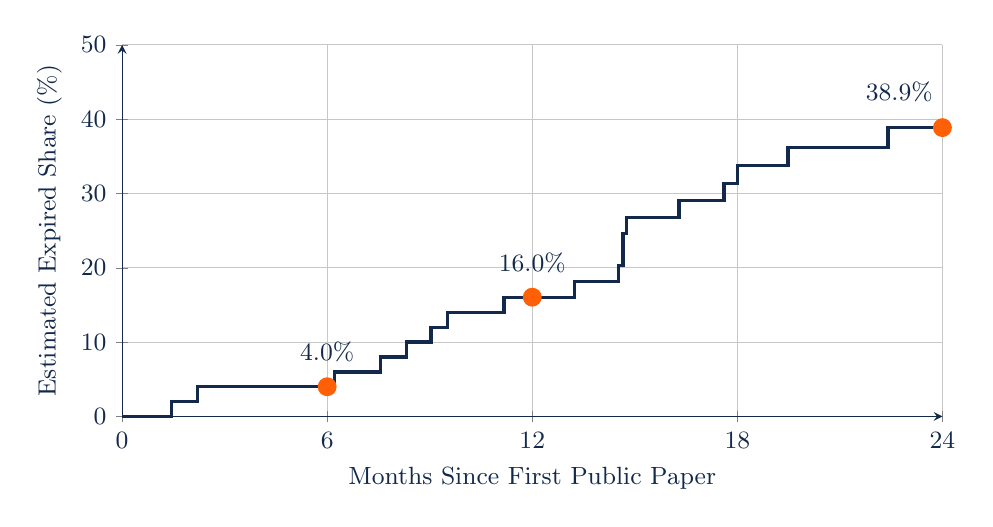
\begin{tikzpicture}
\begin{axis}[width=12cm,height=6.3cm,xmin=0,xmax=24,ymin=0,ymax=50,
xtick={0,6,12,18,24},ytick={0,10,20,30,40,50},
xlabel={Months Since First Public Paper},ylabel={Estimated Expired Share (\%)},
xmajorgrids=true,ymajorgrids=true]
\addplot[IlliniBlue,very thick,const plot] coordinates {(0.0,0.0) (1.4455852156057496,2.0000000000000018) (2.2012320328542097,4.0000000000000036) (6.209445585215605,6.000000000000005) (7.5564681724846,8.000000000000007) (8.31211498973306,10.000000000000009) (9.034907597535934,12.00000000000001) (9.527720739219713,14.000000000000012) (11.104722792607802,14.000000000000012) (11.170431211498974,16.047619047619065) (11.958932238193018,16.047619047619065) (13.240246406570842,18.20024420024422) (14.521560574948666,20.352869352869373) (14.652977412731007,24.65811965811968) (14.751540041067761,26.810744810744836) (15.671457905544148,26.810744810744836) (16.295687885010267,29.028601028601052) (16.361396303901437,29.028601028601052) (16.722792607802873,29.028601028601052) (17.609856262833677,31.394314327647688) (18.0041067761807,33.76002762669431) (18.858316221765914,33.76002762669431) (19.482546201232033,36.21335993681674) (19.581108829568787,36.21335993681674) (21.913757700205338,36.21335993681674) (22.406570841889117,38.87113660611604) (24.0,38.87113660611604)};
\addplot[only marks,mark=*,IlliniOrange,mark size=3pt] coordinates {(6,4) (12,16.047619047619066) (24,38.87113660611604)};
\node[anchor=south,font=\small] at (axis cs:6,6) {4.0\%};
\node[anchor=south,font=\small] at (axis cs:12,18) {16.0\%};
\node[anchor=south east,font=\small] at (axis cs:24,41) {38.9\%};
\end{axis}
\end{tikzpicture}

\end{adjustbox}
\endgroup
\par\medskip
{\small All fifty claims contribute follow-up; 28 remain right-censored.\par}
\note{The 15.75-month mean conditions on the 22 expired claims. It is not an expected lifetime for all findings. The displayed calculation retains the unexpired claims until the observation endpoint. Interval-based and model-count dates are treated as the authors' point estimates; their uncertainty is not propagated.

Queen and Zou (2026), released fitted dates; original course calculation. \url{../01_Resources/14_LLM_Evidence_and_Revalidation/README.md}}
\end{frame}
\begin{frame}{Energy-Plausibility Screens}
\usebeamercolor[fg]{normal text}
\vfill
\begin{slidebullets}
\item An intake-to-requirement comparison needs defined inputs.
\item Unobserved physiological inputs remain missing.
\item A hypothetical Goldberg calculation teaches the method separately from the logs.
\end{slidebullets}
\vfill
\note{The Goldberg example in the notes is an explicitly hypothetical scenario. Its inputs should not be silently imputed from undocumented codes. Screening validity depends on the instrument and population.

M2, Section 2.11.1, Marketing Analytics Lecture Notes. \url{../06_Lecture_Notes/modules/M02_Customer_Data_and_Visualization.md}}
\end{frame}
\begin{frame}{Interactive Comparisons}
\usebeamercolor[fg]{normal text}
\vfill
\begin{slidebullets}
\item Keep comparable panels on common scales.
\item Display the eligible population and current selection.
\item Preserve customers with no recorded days when the estimand includes them.
\end{slidebullets}
\vfill
\note{Changing a slider can change the population, the denominator, and the axis range simultaneously. These changes should remain visible and should be checked against an aggregate table.

M2, Section 2.15, Marketing Analytics Lecture Notes. \url{../06_Lecture_Notes/modules/M02_Customer_Data_and_Visualization.md}}
\end{frame}
\begin{frame}[fragile]{A Composition Check}
\usebeamercolor[fg]{normal text}
\noindent Synthetic within-group rates are 9\%, 80\%, 10\%, and 81\%.
\begin{lstlisting}
rates_a = [0.09, 0.80]
rates_b = [0.10, 0.81]
common_a = sum(rates_a) / 2
common_b = sum(rates_b) / 2
observed_b = (2 * rates_b[0] + rates_b[1]) / 3
assert round(common_b - common_a, 2) == 0.01
\end{lstlisting}
{\small B improves by one point under common weights despite its lower observed aggregate.\par}
\note{The observed B mix assigns two-thirds of its customers to the new-customer group. This calculation is descriptive and uses imposed rates.

M2, Section 2.3, Marketing Analytics Lecture Notes. \url{../06_Lecture_Notes/modules/M02_Customer_Data_and_Visualization.md}}
\end{frame}
\begin{frame}{Coding Exercise: A Chart Assessment}
\usebeamercolor[fg]{normal text}
\vfill
\begin{slidebullets}
\item Generate a rate chart from a verified aggregate table.
\item Alter the axis range, cohort filter, and denominator one at a time.
\item Explain which changes alter the substantive comparison.
\end{slidebullets}
\vfill
\note{The small example runs with ../03\_Data\_and\_Code/Lecture\_Examples/session\_examples.py S03. The complete mHealth visualization program and interactive chart provide the real-data extension. Verify values separately from rendered readability.

M2, Section 2.14, Marketing Analytics Lecture Notes. \url{../06_Lecture_Notes/modules/M02_Customer_Data_and_Visualization.md}}
\end{frame}
\begin{frame}{A Public-Signal Measurement Problem}
\usebeamercolor[fg]{normal text}
\vfill
\begin{slidebullets}
\item A product can acquire a new page title while demand stays unchanged.
\item A single-title series then misses part of its recorded attention.
\item Coverage, redirects, and missing dates require an assessment.
\end{slidebullets}
\vfill
\note{Pageviews measure attention to selected pages. They do not directly measure paid demand or unique customers. Alias aggregation also needs checks for duplicate coverage.

M2, Section 2.17, Marketing Analytics Lecture Notes. \url{../06_Lecture_Notes/modules/M02_Customer_Data_and_Visualization.md}}
\end{frame}
\begin{frame}{Title Changes and Apparent Declines}
\usebeamercolor[fg]{normal text}
\centering
\begingroup
\begin{adjustbox}{max width=0.98\textwidth,max totalheight=0.65\textheight}
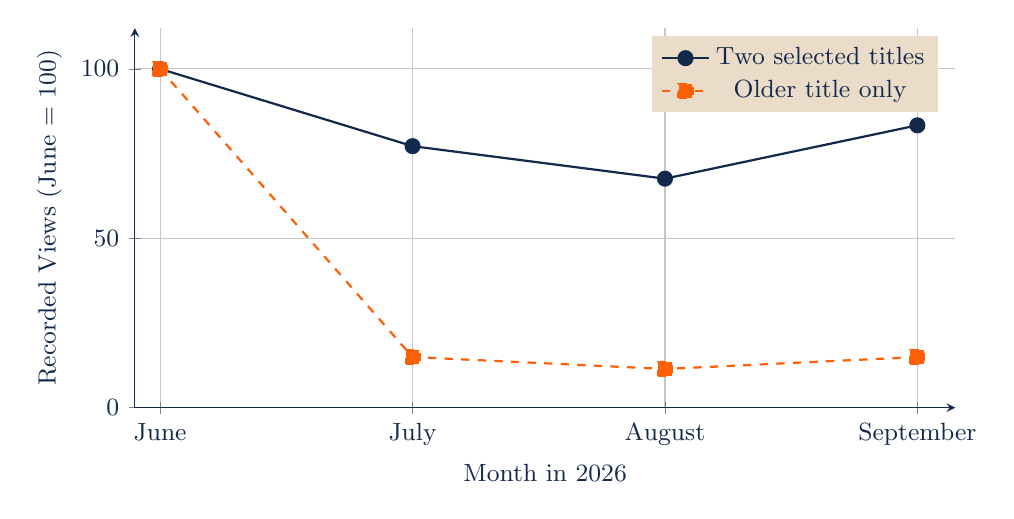
\begin{tikzpicture}
\begin{axis}[width=12cm,height=6.4cm,xmin=-0.1,xmax=3.15,ymin=0,ymax=112,
 xlabel={Month in 2026},ylabel={Recorded Views (June = 100)},
 xtick={0,1,2,3},xticklabels={June,July,August,September},
 legend style={at={(0.98,0.98)},anchor=north east},grid=major]
\addplot[IlliniBlue,mark=*,mark size=2.5pt] coordinates {(0.000000,100.000000) (1.000000,77.188372) (2.000000,67.587098) (3.000000,83.338586)};
\addplot[IlliniOrange,dashed,mark=square*,mark size=2.5pt] coordinates {(0.000000,100.000000) (1.000000,14.939084) (2.000000,11.414054) (3.000000,14.938507)};
\legend{Two selected titles,Older title only}
\end{axis}
\end{tikzpicture}

\end{adjustbox}
\endgroup
\par\medskip
{\small The supplied public pageview capture uses observed title histories.\par}
\note{The GenAI measurement program validates date and title coverage before calculating a product series. Its saved tables are the values behind the plotted comparison.

M2, Section 2.17.1, Marketing Analytics Lecture Notes. \url{../06_Lecture_Notes/modules/M02_Customer_Data_and_Visualization.md}}
\end{frame}
\begin{frame}{Evidence in a Management Presentation}
\usebeamercolor[fg]{normal text}
\vfill
\begin{slidebullets}
\item State the decision and supported result.
\item Show the comparison, units, and denominator.
\item Keep the qualification that could change the action beside the claim.
\end{slidebullets}
\vfill
\note{An executive summary can be concise while retaining consequential uncertainty. A useful chart title states the population and comparison rather than a causal claim unsupported by the design.

M2, Section 2.7, Marketing Analytics Lecture Notes. \url{../06_Lecture_Notes/modules/M02_Customer_Data_and_Visualization.md}}
\end{frame}
\begin{frame}{Honest Comparisons}
\usebeamercolor[fg]{normal text}
\vfill
\begin{slidebullets}
\item Keep denominators and scales visible.
\item Preserve missing outcomes and relevant subgroup variation.
\item Avoid presenting a filtered descriptive pattern as a general causal effect.
\end{slidebullets}
\vfill
\note{A technically correct chart can still communicate a stronger claim than the evidence supports. The reader's likely interpretation matters when selecting a title and comparison.

ETHICS\_AND\_REGULATION.md, M2-M3.}
\end{frame}
\begin{frame}{Visualization Discussion}
\usebeamercolor[fg]{normal text}
\vfill
\begin{slidebullets}
\item Which customers receive weight in the chart?
\item Could sample restrictions reverse the recommendation?
\item What does the uncertainty interval include?
\end{slidebullets}
\vfill
\note{The answers should identify whether the unit is an event, a day, or a customer. Sensitivity to inclusion rules can indicate that the decision depends on a narrower population than the headline suggests.

M2, Section 2.8, Marketing Analytics Lecture Notes. \url{../06_Lecture_Notes/modules/M02_Customer_Data_and_Visualization.md}}
\end{frame}
\end{document}
